\chapter{Method}
\section{Estimating hydrological component from datasets}\label{section:combine}
As mentioned before, the terrestrial water balance can be written as:
\begin{equation}
P - ET - R = \frac{dS}{dt}
\end{equation}
where
\begin{table}[htbp]
	\begin{tabular}{ll}
		$P$   & Precipitation    \\ 
		$ET$    & evapotranspiration \\ \
		$R$     & Surface Runoff \\ 
		$dS / dt$ & total water storage change \\ 
	\end{tabular}
\end{table}\\
For each, time series from different resources are processed using different methods\\\\
 Jet Propulsion Laboratory (JPL), Center for Space Research (CSR), German Research Centre for Geosciences (GFZ) and Institute of Theoretical Geodesy and Satellite Geodesy (ITSG)  post process Level-1 data of GRACE and provide solutions in terms of spherical harmonics. It should be noted that there is a one-year gap between the GRACE and GRACE-FO and several monthly gaps. This one-year gap would be ignored since we are interested in the long term trend and these monthly gaps are dealt using interpolation. For the equivalent water height we use spline interpolation while for uncertainty we use linear interpolation.\\\\
If two known points are given by the coordinates $(x_0,y0)$ and $(x_1,y_1)$, the linear interpolant is the straight line between these points. For a value $x$ in the interval $(x_0,x_1)$, the value $y$ along the straight line is given from the equation of slopes.
\begin{equation}
	y = y_0 + (x-x_0)\frac{y_1-y_0}{x_1-x_0}
\end{equation}
Spline was a term of elastic rulers that were bent to pass through a number of predifined points (knots). The approch to mathematically modelling the shape of such elastic rulers fixed by $n+1$ knots is to interpolate between all the pairs of knots and new point with polynomials. In MatLab, both of these interpolation methods can be finished using function \textit{griddedInterpolant}.\\\\
We have 4 TWSA time series from CSR, GFZ, ITSG and JPL with different uncertainties. To generate one time series of TWSA for further analyse we use Gaus-Markov model.
\subsection{Adjustment using Gauss-Markov model}\label{sec:Gaussmarkov}
Gauss-Markov model is known as the adjustment with observation equations. The model is as follows
\begin{equation}
\bm{y} = \bm{A}\bm{x} + \bm{e}
\end{equation}
where $y$ is a vector of observations, $A$ is the design matrix, $x$ is a vector of unknowns and $e$ is a vector of measurement errors. Define the \textit{Lagrangian} or \textit{cost function};
\begin{equation}
\mathcal{L}_{a}(x) = \frac{1}{2} \bm{e}^T \bm{e}
\end{equation} 
Then, the adjusted observations can be estimated by using least square criterion, the best $x$ can be found with the minimum cost function. The equations can be solved as following:
\begin{align}
&\hat{\bm{x}} = (\bm{A}^T\bm{A})^{-1}\bm{A}^T\bm{y}\\
&\hat{\bm{y}} = \bm{A}\hat{\bm{x}} = \bm{A}(\bm{A}^T\bm{A})^{-1}\bm{A}^T\bm{y}\\
&\hat{\bm{e}} = \bm{y} - \hat{\bm{y}} = [\bm{I} - \bm{A}(\bm{A}^T\bm{A})^{-1}\bm{A}^T]\bm{y}
\end{align}
In many cases, the observations are not equal weighted, which means they have different quality. To solve this problem,  we use a matrix $\bm{P}$ to describe the weight. The cost function is formed as:
\begin{equation}
\mathcal{L}_{a}(x) = \frac{1}{2} \bm{e}^T \bm{P}\bm{e}
\end{equation}
the weighted least squares estimations are:
\begin{align}
\label{equa:guass0}
&\hat{\bm{x}} = (\bm{A}^T \bm{P}\bm{A})^{-1}\bm{A}^T\bm{P}\bm{y}\\ 
&\hat{\bm{y}} = \bm{A}\hat{\bm{x}} = \bm{A}(\bm{A}^T\bm{P}\bm{A})^{-1}\bm{A}^T\bm{P}\bm{y}\\
&\hat{\bm{e}} = \bm{y} - \hat{\bm{y}} = [\bm{I} - \bm{A}(\bm{A}^T\bm{P}\bm{A})^{-1}\bm{A}^T\bm{P}]\bm{y}
\end{align}\\
For each month, their are 4 EWH values $S_{CSR}(t)$, $S_{GFZ}(t)$, $S_{ITSG}(t)$, $S_{JPL}(t)$ along with their uncertainty $\sigma_{CSR}(t)$, $\sigma_{GFZ}(t)$, $\sigma_{ITSG}(t)$, $\sigma_{JPL}(t)$. We use the uncertainty to build the weight matrix $\bm{P}$, then we have:
\begin{align}
\bm{y} &= \begin{pmatrix} \label{equa:guass1}
S_{CSR}(t)\\
S_{GFZ}(t)\\
S_{ITSG}(t)\\
S_{JPL}(t)
\end{pmatrix} \\
\bm{P} &= \begin{pmatrix} \label{equa:guass2}
\frac{1}{\sigma^2_{CSR}(t)} & 0 & 0 & 0 \\
0 & \frac{1}{\sigma^2_{GFZ}(t)} & 0 & 0 \\
0 & 0 & \frac{1}{\sigma^2_{ITSG}(t)} & 0 \\
0 & 0 & 0 & \frac{1}{\sigma^2_{JPL}(t)}
\end{pmatrix}\\
\bm{A} &= \begin{pmatrix} \label{equa:guass3}
1\\
1\\
1\\
1
\end{pmatrix}
\end{align}
By inserting \autoref{equa:guass1}, \autoref{equa:guass2} and \autoref{equa:guass3} into \autoref{equa:guass0} we are able to get one TWSA for one month
\begin{equation} \label{equa:finalgauss}
\underset{1 \times 1}{\hat{\bm{x}}} = (\underset{1 \times 4}{\bm{A}}^T \underset{4 \times 4}{\bm{P}} \  \underset{4 \times 1}{\bm{A}})^{-1} \underset{1 \times 4}{\bm{A}}^T \underset{4 \times 4}{\bm{P}} \  \underset{4 \times 1}{\bm{y}}
\end{equation}
where $\hat{\bm{x}}$ is the EWH for one month. By repeating \autoref{equa:finalgauss}, we are able to get one whole time series for equivalent water height. The uncertainty for this new time series would be calculated using least squares error:
\begin{equation}
	\sigma(t) = \frac{1}{4}\sqrt{\sigma^2_{CSR}(t)+\sigma^2_{GFZ}(t)+\sigma^2_{ITSG}(t)+\sigma^2_{JPL}(t)}
\end{equation}
The derivation of the TWSA would be calculated using central difference:
\begin{align}\label{eq:dsdt}
\frac{dS(t)}{dt} = &\frac{(dS(t+\Delta t) - dS(t)) + (dS(t) - dS(t-\Delta t))}{2 \Delta t}\\
= & \frac{dS(t+\Delta t) - dS(t-\Delta t)}{2 \Delta t}
\end{align}
where $\Delta t$ is one month. 
The method used in \autoref{sec:Gaussmarkov} also works for precipitation, evapotranspiration and runoff. However, the uncertainties of these time series were unknown. Therefor, it's necessary to get the uncertainty before the adjustment. \\\\
We assume that the precipitation and evapotranspiration are normal distributed during 2002 to 2020 (though it is not the case). Under this assumption, the precipitation and evapotranspiration in the same month every year can be regarded as a constant with random errors. We then can use the standard deviation as the uncertainty.
\begin{gather}
\sigma_{Pre_{Jan}} = \sqrt{\frac{\sum_{i=1}^{n} (Pre(i)_{Jan} - \bar{Pre}_{Jan})}{n-1}}
\end{gather}
where $\sigma_{Pre_{Jan}}$ is the standard deviation of the Precipitation in January, $Pre(i)_{Jan}$ is the precipitation in January in different years and $\bar{Pre}_{Jan}$ is the mean of all the precipitation in January. With the same method we are able to obtain the uncertai nty for precipitation and evapotranspiration in other eleven months. \\\\
The changing points can be found using moving average (MA). In statistics, a moving average is a calculation used to analyze data points by creating a series of averages of different subsets of the full data set. The reason for calculating the moving average is to help smooth out the data by creating a constantly updated average data. In MatLab, this could be down with \textit{movmean} function. The size of subsets is 12 in this thesis because of the number of months in one year.\\\\
After moving average time series the abrupt changes in the mean of the this new series, the sudden change of the time series can be found. This can be achieved using MatLab function \textit{ischange}, which enables user to find the abrupt changes of the a vector in mean value, variance or sloe and intercept. 
\section{Estimating the quality of runoff datasets}\label{sec:runoffdata}
It was mentioned in \autoref{sec:runoff} that the in-situ runoff data existed til 2010, which allows us to estimate the quality of the data models. First, we calculate the diFference between the model and the in-situ data.
\begin{equation}
	d(t) = R(t)_{insitu} - R(t)_{model}
\end{equation}
By plotting the cumulative distribution function (CDF) of $d$, the quality of the model can be estimated. By setting the appropriate quantile we are able to decide if a data model is good enough for further analyze. In this work 10\% of the mean in-situ data are set.  
\section{Estimating the runoff using quantile function and water level}\label{sec:waterlevel}
The river discharge at the selected gauges is typically determined from an empirical functional relation between water level estimated by satellite altimetry and measured discharges. This relation, referred to as a rating curve, is specific to each gauging station and location of altimetry. However, this technique has many limitations. First, first, this technique is limited by the availability of in situ discharge measurements simultaneous with altimetry data. Second, the location of the altimetry foot- print can also limit the usage of the technique.\\\\
Fortunately, \cite{tourian2013quantile} provides a methods, which can represent a direct connection between the quantile functions at the corresponding probability and the relationship between runoff and water level. \\\\
first, we get the quantile functions for altimetric water level,$Q_R(p)$ and discharge from in situ measurement, $Q_W(p)$:
\begin{gather*}
	Q_R(p) = \inf(X_R \in R: p\leq F(X_R)) \\
	Q_W(p) = \inf(X_W \in R: p\leq F(X_W)) 
\end{gather*}
where $X_R$ and $X_W$ refer to the runoff and water level values and $F$ represents the CDF. The quantile function specifies, for a given probability $0 < p < 1$, the maximum value that $X_R$ or $X_W$ can attain with that probability.\\\\
By achieving the function $T$ between the quantile functions, we can get the function between the runoff and water level since $T$ is a non decreasing function. 
\begin{equation}
	Q_R = T(Q_W) \Longrightarrow X_R = T(X_W)
\end{equation}
In principle, the obtained relationship can be used as look-up table implying the desired rating curve. However, as this study aims to compare the statistical and empirical rating curves, a similar way of approximation for both is needed. In this thesis, the simple quadratic estimation is used for modeling the rating curve. Thus, the statistical rating curve is achieved by fitting a quadratic curve over the obtained statistical relationship. \autoref{fig:wltodischarge} showed an example of achieving the runoff using water level data from Envisat. 
\begin{figure}[htbp]
	\centering
	\begin{minipage}[t]{0.45\textwidth}
		\centering
		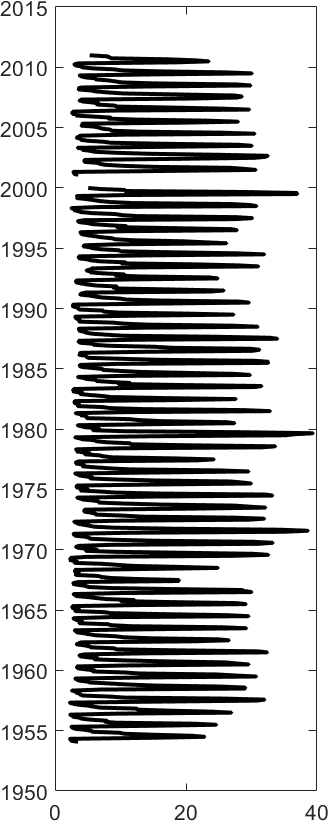
\includegraphics[width=0.4\textwidth]{leftinsitu} % Datei in "bilder/" bei LaTeX: eps, bei PDFLaTeX: jpg (o.ä.) 
	\end{minipage}
	\begin{minipage}[t]{0.45\textwidth}
		\centering
		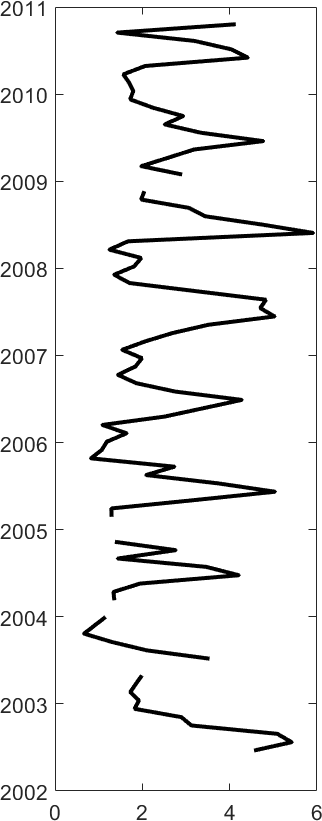
\includegraphics[width=0.4\textwidth]{rightwl} % Datei in "bilder/" bei LaTeX: eps, bei PDFLaTeX: jpg (o.ä.) 
	\end{minipage}
	\begin{minipage}[t]{0.45\textwidth}
		\centering
		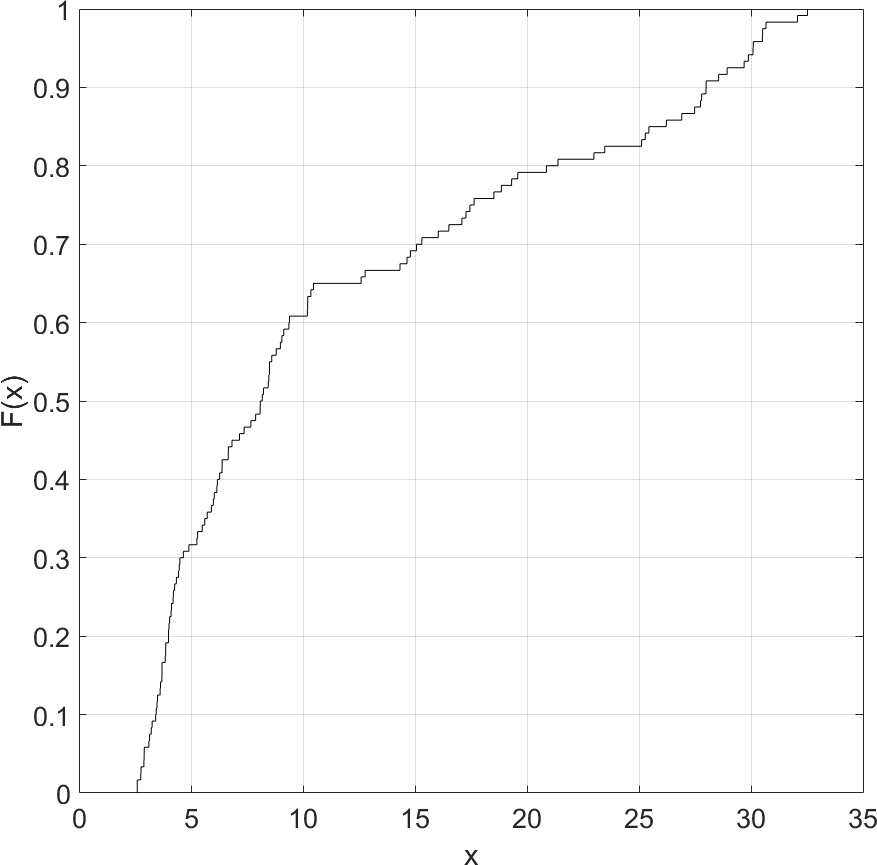
\includegraphics[width=0.7\textwidth]{cdfleft} % Datei in "bilder/" bei LaTeX: eps, bei PDFLaTeX: jpg (o.ä.) 
	\end{minipage}
	\begin{minipage}[t]{0.45\textwidth}
		\centering
		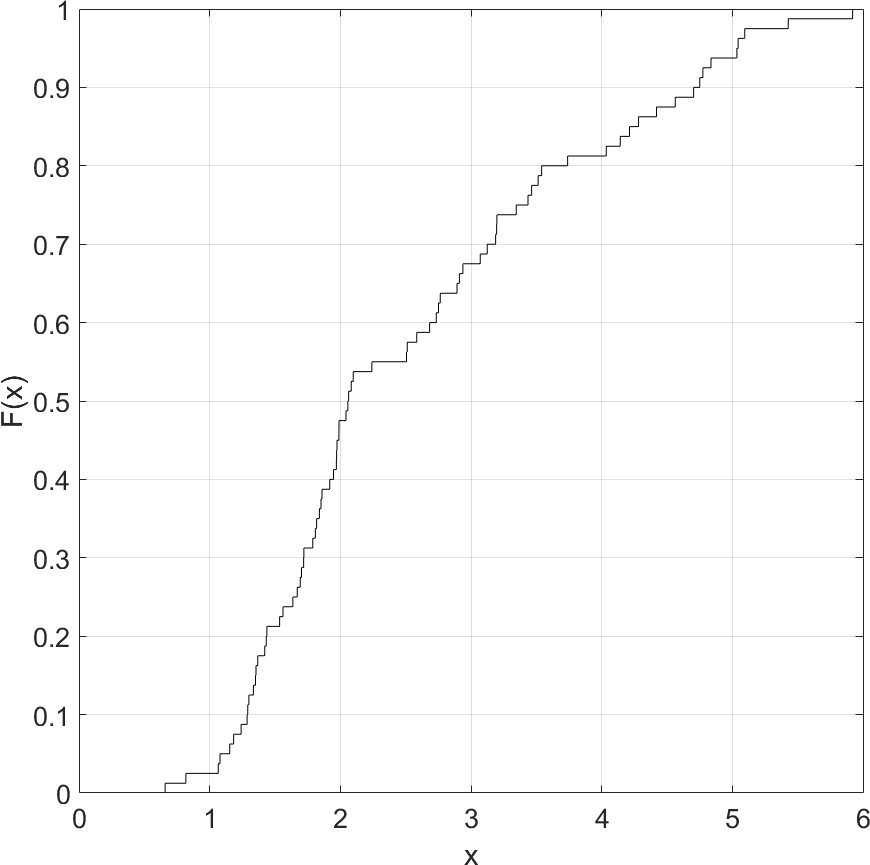
\includegraphics[width=0.7\textwidth]{cdfright} % Datei in "bilder/" bei LaTeX: eps, bei PDFLaTeX: jpg (o.ä.) 
	\end{minipage}
	\begin{minipage}[t]{0.45\textwidth}
		\centering
		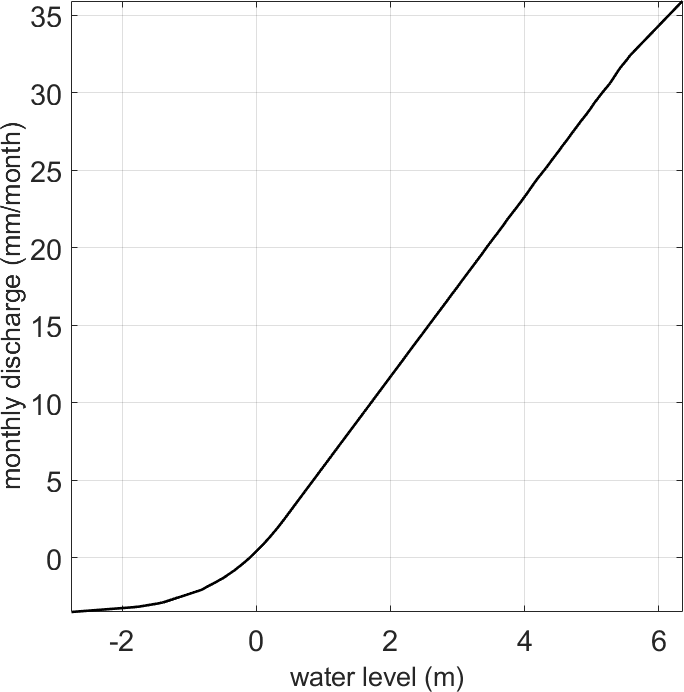
\includegraphics[width=0.7\textwidth]{cdfcombine} % Datei in "bilder/" bei LaTeX: eps, bei PDFLaTeX: jpg (o.ä.) 
	\end{minipage}
	\caption{Available in-situ runoff for Ob river (top left), stimatEd water level from Envisat (top right), and quantile function of water level and runoff (middle). A smoothened rating curve is obtained from the corresponding probabilities (bottom)}
	\label{fig:wltodischarge}
\end{figure}\\\\
By repeating this process to SARAL and Sentinel missions we can generate an whole runoff time series from 2002 to 2020. (note there is a 32 months gap between Envisat and SARAL from November of 2010 to July of 2013) 